\chapter{Lecture 13: More Contour Integration}

\begin{example}
    Find the value of:
    $$\int_{0}^{\infty} \frac{x^{1/3}}{x^2 + 4x + 8} dx$$

    \textbf{step 1:} Replace with a complex function:
    Let $f(z) = \frac{z^{1/3}}{z^2 + 4z + 8}$, then:
    \begin{align*}
        \int_{0}^{\infty} \frac{x^{1/3}}{x^2 + 4x + 8} dx & = \int_{-\infty}^{\infty} \frac{z^{1/3}}{z^2 + 4z + 8} dz             \\
                                                          & = \int_{-\infty}^{\infty} \frac{e^{\frac{1}3\log z}}{z^2 + 4z + 8} dz
    \end{align*}

    \textbf{step 2:} Choose the right contour:
    \textbf{NOTE: } $\int_{-\infty}^{0} \frac{|z|^{1/3}}{z^2 + 4z + 8} dz \neq \int_{0}^{\infty} \frac{z^{1/3}}{z^2 + 4z + 8} dz$ so, $\int_{-\infty}^{\infty} \frac{z^{1/3}}{z^2 + 4z + 8} \neq 2\int_{0}^{\infty} \frac{x^{1/3}}{x^2 + 4x + 8} dx$ because $z^2 + 4x + 8$ is not even.
    (There's an absolute value in the numerator because we'd be able to evaluate the imaginary part of the logarithm explicitly)
    Therefore a half-keyhole contour is not appropriate. We can use a full keyhole contour as seen in the figure below.

    \begin{figure}[H]
        \centering
        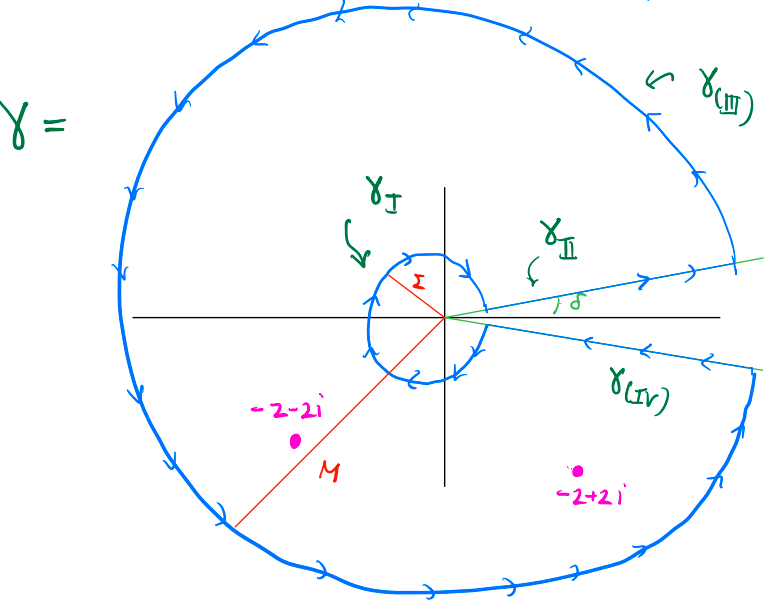
\includegraphics[width=0.75\textwidth]{LECTURE_13/keyhole-contour.png}
    \end{figure}

    \textbf{Step 2.5:} Choose the branch cut:
    We need to choose a branch cut over which $z^{1/3}$ is analytic. We can choose the positive real axis so that $\arg(z) \in [0, 2\pi)$.

    \textbf{step 3:} If there are singularities in the contour, find their residues:
    There are singularities at $z = -2 \pm 2i$. They are both enclosed by the contour, so we need to find the residues at both points. We can write:
    \begin{align*}
        \rightarrow f(z)                   & = \frac{z^{1/3}}{(z + 2 - 2i)(z + 2 + 2i)}                                      \\
        \text{Res}(f,z_k)                  & = \lim_{z \to z_k} (z - z_k) f(z)                                               \\
        \text{Res}(f,-2 + 2i)              & = \lim_{z \to -2 + 2i} (z - (-2 + 2i)) \frac{z^{1/3}}{(z + 2 - 2i)(z + 2 + 2i)} \\
                                           & = \lim_{z \to -2 + 2i} \frac{z^{1/3}}{(z + 2 - 2i)}                             \\
                                           & = \frac{(-2 + 2i)^{1/3}}{(-2 + 2i + 2 - 2i)}                                    \\
                                           & = \frac{2^{1/3}e^{i\pi/4}}{4} = \frac{e^{i\pi/4}}{2^{2/3}}                      \\
        \text{Res}(f,-2 - 2i)              & = \lim_{z \to -2 - 2i} (z - (-2 - 2i)) \frac{z^{1/3}}{(z + 2 - 2i)(z + 2 + 2i)} \\
                                           & = \lim_{z \to -2 - 2i} \frac{z^{1/3}}{(z + 2 + 2i)}                             \\
                                           & = \frac{(-2 - 2i)^{1/3}}{(-2 - 2i + 2 + 2i)}                                    \\
                                           & = \frac{2^{1/3}e^{-i\pi/4}}{4} = \frac{e^{-i\pi/4}}{2^{2/3}}                    \\
        \therefore \text{Res}(f,-2 \pm 2i) & = \frac{e^{\pm i\pi/4}}{2^{2/3}}
    \end{align*}
    We can compute the integral:
    \begin{align*}
        i\pi/4\int_{\gamma_{M,\epsilon,\delta}} f(z)dz & = 2\pi i \left( \frac{e^{i\pi/4}}{2^{2/3}} + \frac{e^{-i\pi/4}}{2^{2/3}} \right) \\
    \end{align*}
    \textbf{step 4:} Find the consequences of the contour:
    Recall Example \ref{ex:keyhole} From chapter 5, lecture 4 for the parametrization of the keyhole contour:
    \begin{align*}
        \gamma (t) = \begin{cases}
                         Me^{i\theta}          & \delta \leq \theta \leq 2\pi - \delta \\
                         te^{i(2\pi - \delta)} & M \leq t \leq \epsilon                \\
                         \epsilon e^{i\theta}  & 2\pi - \delta \leq \theta \leq \delta \\
                         te^{i\delta}          & \epsilon \leq t \leq M
                     \end{cases}
    \end{align*}
    From the residue theorem and the contour in the figure above, we can write:
    \begin{align*}
        i\pi/4\int_{\gamma_{M,\epsilon,\delta}} f(z)dz & = \int_{\gamma_I} f(z)dz + \int_{\gamma_{II}} f(z)dz + \int_{\gamma_{III}} f(z)dz + \int_{\gamma_{IV}} f(z)dz
    \end{align*}
    By previous arguments, as $M \to \infty$ and $\epsilon \to 0$, we can write:
    \begin{align*}
        \int_{\gamma_{I}} f(z)dz   & = 0 \\
        \int_{\gamma_{III}} f(z)dz & = 0 \\
    \end{align*}
    The other two integrals can be computed as:
    \begin{align*}
        \int_{\gamma_{II}} f(z)dz & = \int_{\epsilon}^{M} f(r e^{i\delta})r i e^{i\delta} dr                                                              \\
                                  & = \int_{\epsilon}^{M} \frac{r^{1/3}e^{i\delta/3}}{(r e^{i\delta} + 2 - 2i)(r e^{i\delta} + 2 + 2i)}r i e^{i\delta} dr \\
                                  & \text{As } M \to \infty, \epsilon \to 0, \delta \to 0                                                                 \\
                                  & = \int_{0}^{\infty} \frac{r^{1/3}}{(r + 2 - 2i)(r + 2 + 2i)}r i dr                                                    \\
    \end{align*}
    On the other hand:
    \begin{align*}
        \int_{\gamma_{IV}} f(z)dz & = \int_{M}^{\epsilon} f(r e^{i\delta})r i e^{i\delta} dr                                                                                              \\
                                  & = \int_{M}^{\epsilon} \frac{r^{1/3}e^{i(2\pi -\delta)/3}}{(r e^{i(2\pi -\delta)} + 2 - 2i)(r e^{i(2\pi -\delta)} + 2 + 2i)}r i e^{i(2\pi -\delta)} dr \\
                                  & \text{As } M \to \infty, \epsilon \to 0, \delta \to 0                                                                                                 \\
                                  & = \int_{\infty}^{0} \frac{r^{1/3}e^{i2\pi/3}}{(r + 2 + 2i)(r + 2 - 2i)}r i dr                                                                         \\
                                  & = e^{i2\pi/3}\int_{0}^{\infty} \frac{r^{1/3}}{(r + 2 - 2i)(r + 2 + 2i)}r i dr                                                                         \\
    \end{align*}
    Therefore:
    \begin{align*}
        \left[\int_{0}^{\infty} \frac{r^{1/3}}{(r + 2 - 2i)(r + 2 + 2i)}r i dr\right]\left[1 - e^{i2\pi/3}\right] & = i\pi/4\int_{\gamma_{M,\epsilon,\delta}} f(z)dz                                                         \\
        \int_{0}^{\infty} \frac{r^{1/3}}{(r + 2 - 2i)(r + 2 + 2i)}r i dr                                          & = \frac{2\pi i}{1 - e^{i2\pi/3}} \left( \frac{e^{i\pi/4}}{2^{2/3}} + \frac{e^{-i\pi/4}}{2^{2/3}} \right) \\
    \end{align*}
\end{example}

\begin{proposition}
    [Keyhole Contour Integral]
    Use a keyhole contour to evaluate real integrals with logarithms or fractional powers where the integrand is not even.
    $$\left[\int_{0}^{\infty} f(x)dx\right](1 - e^{i\theta}) = \int_{\gamma_{M,\epsilon,\delta}} f(z)dz = 2\pi i \sum \text{Res}(f,z_k)$$
    Where $\gamma_{M,\epsilon,\delta}$ is the sum of the residues of the singularities enclosed by the contour. $\theta = i\arg z \times \text{fractional power of z}$ for a fractional power of $z$.
\end{proposition}

\section{Analytic Functions as Mappings (Chap. 3)}

\subsection{3.1 - The Zeroes of an Analytic Function}

\begin{lemma}
    Recall that if $f(z)$ is not identically $0$ on a domain $D$ and $f(z_0) = 0$ for some $z_0 \in D$, then $f(z)$ has a pole at $z_0$ of order $m$ if $f(z) = (z - z_0)^m g(z)$ where $g(z)$ is analytic and $g(z_0) \neq 0$.
\end{lemma}

\begin{proposition}
    [The Identity Theorem]
    If $f(z)$ is analytic on a domain $D$ and there exists a sequence of points $\{z_n\}$ in $D$ such that $f(z_n) = 0$ and $z_n \to z_0 \in D$, then $f(z) = 0$ for all $z \in D$.
    \textbf{Alternatively:}
    If $f$ is analytic on $D$, not identically zero, and $f(z_0) = 0$ for some $z_0 \in D$, then $\exists \delta > 0 | z_0$ is the only zero of $f \in \{z \in D | |z - z_0| < \delta\}$.
\end{proposition}

\begin{proof}
    Suppose $f$ is analytic, $f(z_0) = $ and $\exists z_n \in \{|z_0 - z| < \frac{1}n\}$ such that $f(z_n) = 0$ this would mean:
    \begin{align*}
        f(z)   & = \sum_{n=0}^{\infty} a_n(z - z_0)^n               \\
        f(z_0) & = a_0(z_0 - z_0)^0 + a_1(z_0 - z_0)^1 + \ldots = 0
               & = a_0\times 0^0                                    \\
        0 = a_0 \times 1
    \end{align*}
    If $a_0, a_1, \ldots a_{n-1}$ are all $0$ then:
    \begin{align*}
        g(z)   & = \frac{f(z)}{(z - z_0)^n} = a_n + a_{n+1}(z - z_0) + \ldots = 0 \\
        g(z_n) & = \frac{f(z_n)}{(z_n - z_0)^n} = \frac{0}{(z_n - z_0)^n} = 0     \\
        a_n = 0
    \end{align*}
\end{proof}
\begin{figure}[H]
    \centering
    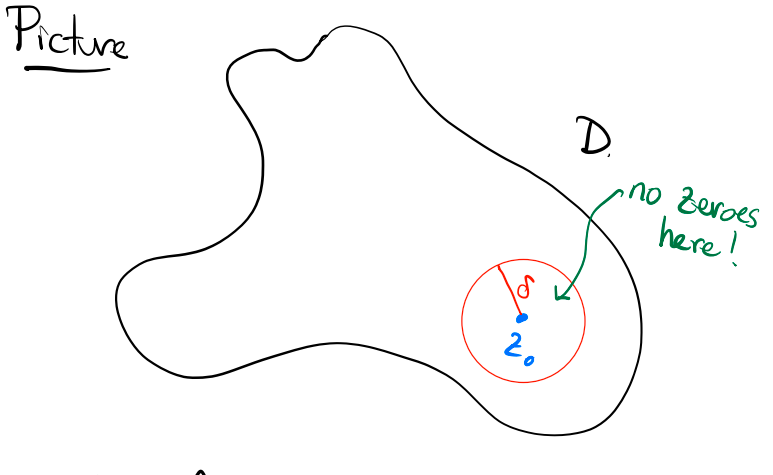
\includegraphics[width=0.75\textwidth]{LECTURE_13/pic.png}
    \caption{$\delta$ where no other zeroes exist}
\end{figure}

\begin{proposition}
    If $D$ is a bounded domain (i.e. $D \subset \{|z| < M\}$ for some $M$) then $f$ has only finitely many zeroes. Thus, we can count them. This can be done using the residue theorem.
\end{proposition}

\begin{proof}
    Zeroes are isolated in $D$ so they must be at least some $\delta$ apart. If $D$ then there is only finite space for zeroes and thus, there are only finitely many zeroes.
\end{proof}

\begin{theorem}
    [Argument Principle]
    Suppose $h$ is analytic in a domain $D$ except for a finite number of isolated poles. Let $\gamma$ be a piecewise $C^{1}$, positively oriented, simple closed curve in $D$, which does not pass through any pole or zero of $h$, and such that inside$(\gamma) \subset D$. Then:
    $$\frac{1}{2\pi i}\int_{\gamma} \frac{h'(z)}{h(z)}dz = \text{number of zeroes of } h \text{ inside } \gamma - \text{number of poles of } h \text{ inside } \gamma$$
    $$
        \frac{1}{2\pi}
        \left\{
        \begin{aligned}
             & \text{change in } \arg h(z)            \\
             & \text{as } z \text{ traverses } \gamma
        \end{aligned}
        \right\}
        =
        \left\{
        \begin{aligned}
             & \text{no. of zeros of } h \\
             & \text{inside } \gamma
        \end{aligned}
        \right\}
        -
        \left\{
        \begin{aligned}
             & \text{no. of poles of } h \\
             & \text{inside } \gamma
        \end{aligned}
        \right\}.
    $$

    Where all zeroes and poles are counted with their multiplicities.
\end{theorem}

\begin{example}
    The function $z^k$ has $k$ zeroes inside the unit circle and $k$ poles outside of it.
\end{example}

\begin{proof}
    $\frac{h'(z)}{h(z)}$ is analytic except at zeroes or poles of $h$.
    If $h$ has a zero of order $k$ at $z_0$, then $h = (z - z_0)^kg(z) \quad g(z) \text{ analytic } g(z_0) \neq 0$. so:
    \begin{align*}
        \frac{h'}{h} & = \frac{k(z - z_0)^{k-1}g(z) + (z - z_0)^kg'(z)}{(z - z_0)^kg(z)}                 \\
                     & = \frac{k}{z - z_0} + \underbrace{\frac{g'(z)}{g(z)}}_{\text{analytic near } z_0}
    \end{align*}
    Thus:
    \begin{align*}
        \text{Res}(h'/h,z_0) & = k = \text{order of zero at } z_0
    \end{align*}
    Now if $h$ has a pole order $k$ at $z_0$ then $h = \frac{H(z)}{(z - z_0)^k} \quad H(z) \text{ analytic } H(z_0) \neq 0$. so:
    \begin{align*}
        \frac{h'}{h} & = \left[\frac{H'(z)}{(z - z_0)^k} - \frac{kH(z)}{(z - z_0)^{k+1}}\right]\frac{(z - z_0)^{k}}{H(z)} \\
                     & = -\frac{k}{z - z_0} + \underbrace{\frac{H'(z)}{H(z)}}_{\text{analytic near } z_0}
    \end{align*}
    Thus:
    \begin{align*}
        \text{Res}(h'/h,z_0) & = -k = \text{order of pole at } z_0
    \end{align*}
    We can conclude that:
    \begin{align*}
        \frac{1}{2\pi i}\int_{\gamma} \frac{h'(z)}{h(z)}dz & = \sum_{z_j \text{ zeroes } h} \text{order of zeroes at }z_j - \sum_{z_k \text{ poles } h} \text{order of poles at }z_k \\
                                                           & = \text{number of zeroes of } h \text{ inside } \gamma - \text{number of poles of } h \text{ inside } \gamma
    \end{align*}
\end{proof}

\begin{example}
    Consider $h(z) = z^k$, and the curve $\gamma = e^{i\theta}$ then:
    \begin{figure}[H]
        \centering
        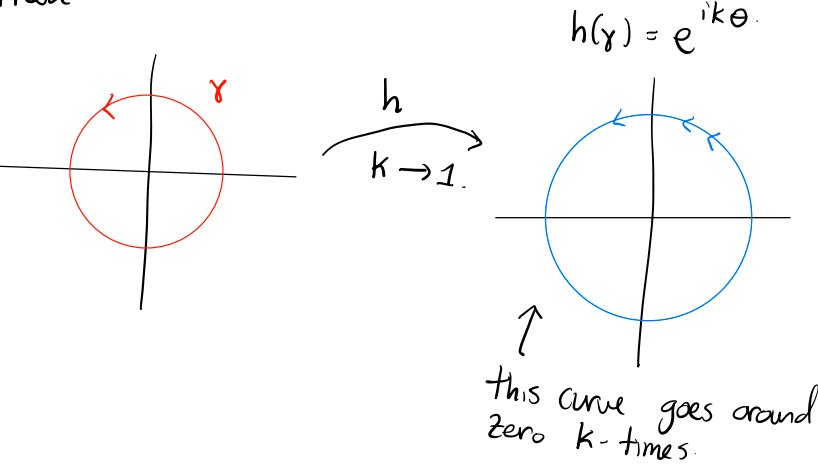
\includegraphics[width=0.75\textwidth]{LECTURE_13/gamma.png}
        \caption{The curve $\gamma$}
    \end{figure}

    \textbf{Step 1:} find $h'(z)/h(z)dz$:
    \begin{align*}
        \frac{h'(z)}{h(z)} & = d\log h(z) \text{ By definition}                                                                     \\
                           & = \underbrace{d\log|h|}_{\text{change in }|h(z)|} + \underbrace{id\theta}_{\text{change in }\arg h(z)} \\
                           & = dr + id\theta
    \end{align*}
    So:
    \begin{align*}
        \int_{\gamma} \frac{h'(z)}{h(z)}dz & = \int_{h(\gamma)} dr + id\theta                                          \\
                                           & = \log\frac{|h(\gamma(2\pi))|}{|h(\gamma(0))|} + i(\arg h(\gamma(2\pi)))k \\
                                           & = 0 _ i2\pi k
    \end{align*}
    Similarly if $h(z) = \frac{1}{z^k}$ then:
    \begin{figure}[H]
        \centering
        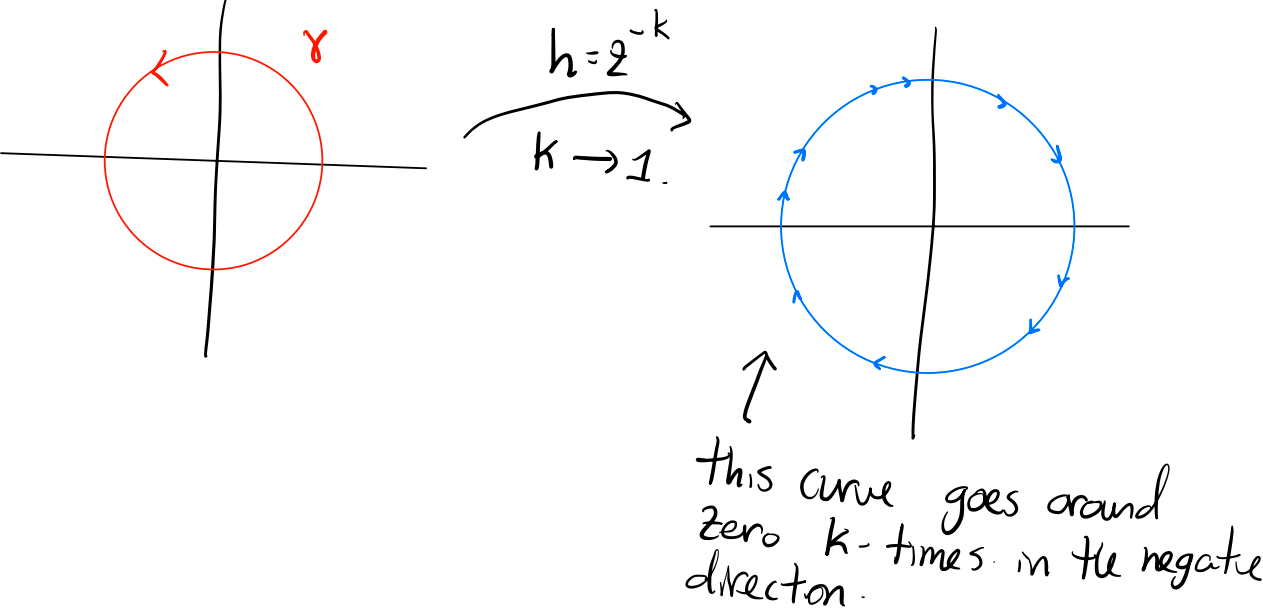
\includegraphics[width=0.75\textwidth]{LECTURE_13/gamma_rev.png}
        \caption{The reverse curve $\gamma$}
    \end{figure}

\end{example}

\begin{example}
    Find the number of zeroes of $f(z) = z^3 - 2z^2 + 4$ in the first quadrant
    \begin{figure}[H]
        \centering
        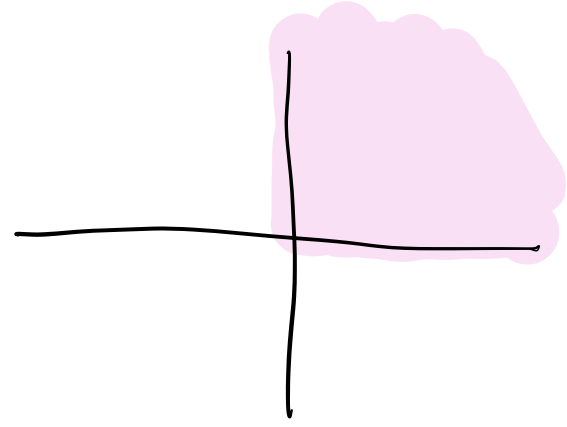
\includegraphics[width=0.75\textwidth]{LECTURE_13/first-quadrant.png}
        \caption{The first quadrant}
    \end{figure}

    \textbf{Solution:}
    \textbf{Step 1:} Consider the contour
    \begin{figure}[h]
        \centering
        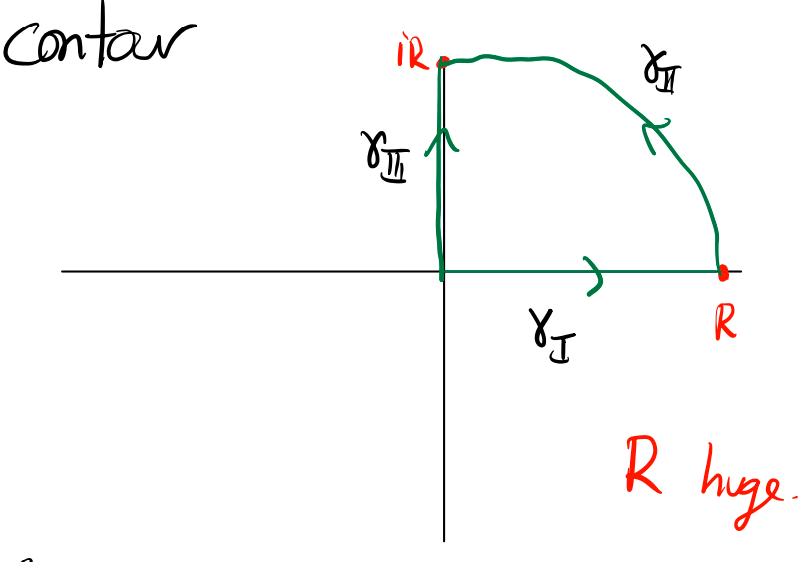
\includegraphics[width=0.75\textwidth]{LECTURE_13/first-quadrant-contour.png}
        \caption{The contour}
    \end{figure}
    \textbf{Step 2:} Find $\Delta \arg f(\gamma_k) \forall k$
    \begin{align*}
        \gamma_I & = x \quad t \in [0, R] \quad \rightarrow\quad f(\gamma_I) = t^3 - 2t^2 + 4
    \end{align*}
    This is a real function, so as long as $f(\gamma_I) \geq 0$ from $t = 0$ to $t = R$, then $\Delta \arg f(\gamma_I) = 0$. We know this function will have a minimum at $f'(t)$
    \begin{align*}
        f'                       & = 3t^2 - 4t = x(3x - 4)                                                                                                  \\
        \rightarrow f(0)         & = 4                                                                                                                      \\
        \rightarrow f(\frac{4}3) & = t^3 - 2t^2 + 4 = \frac{64}{27} - \frac{32}{9} + 4 = \frac{64}{27} - \frac{96}{27} + \frac{108}{27} = \frac{76}{27} > 0
    \end{align*}
    So $\Delta \arg f(\gamma_I) = 0$.
    \begin{align*}
        \gamma_{II}    & = Re^{i\theta}\quad \theta \in [0, \pi/2]                                             \\
        f(\gamma_{II}) & = R^3e^{3i\theta} - 2R^2e^{2i\theta} + 4                                              \\
                       & = R^3e^{3i\theta}\left(1 - \frac{2}{R}e^{i\theta} + \frac{4}{R^3}e^{-3i\theta}\right) \\
                       & \text{As } R \to \infty                                                               \\
                       & = R^3e^{3i\theta}
    \end{align*}
    $R$ is the magnitude of the function, complex exponential function gives the argument of the function.
    \begin{align*}
        e^{ig(\theta)} \rightarrow g(\theta) = \arg f(\gamma_{II}) = 3\theta
    \end{align*}
    Because $\theta \in [0, \pi/2]$ then $\Delta \arg f(\gamma_{II}) = 3\pi/2$.
    \begin{align*}
        \gamma_{III}    & = iy \quad \rightarrow\quad t \in [0, R] \\
        f(\gamma_{III}) & = iy^3 + 2y^2 + 4                        \\
    \end{align*}
    We know the argument of a function is given by $\tan^{-1}(\frac{\Im(f)}{\Re(f)})$
    \begin{align*}
        \arg f(\gamma_{III})_1 & = 0 \quad \text{because } f(\gamma_{III}(0)) = 4 \\
    \end{align*}
    Because the function begins on the real axis when $t = 0$, the argument is $0$.
    \begin{align*}
        \arg f(\gamma_{III})_2                 & =\lim_{y= R\to \infty} \tan^{-1}\left(\frac{y^3}{2y^2 + 4}\right) \\
                                               & = tan^{-1}(\inf) = \frac{\pi}2                                    \\
        \therefore \Delta \arg f(\gamma_{III}) & = \frac{\pi}2
    \end{align*}
    So all together:
    \begin{align*}
        \Delta \arg f(\gamma) & = \Delta \arg f(\gamma_I) + \Delta \arg f(\gamma_{II}) + \Delta \arg f(\gamma_{III}) \\
                              & = 0 + \frac{3\pi}2 + \frac{\pi}2 = 2\pi
    \end{align*}
    We notice that $f$ has no poles in the first quadrant, so by the argument principle:
    \begin{align*}
        \frac{1}{2\pi}\left\{\begin{aligned}
                                  & \text{change in } \arg h(z)            \\
                                  & \text{as } z \text{ traverses } \gamma
                             \end{aligned}\right\} + \left\{\begin{aligned}
                                                                 & \text{no. of poles of } h \\
                                                                 & \text{inside } \gamma
                                                            \end{aligned}\right\} & = \left\{\begin{aligned}
                                                                                                  & \text{no. of zeros of } h \\
                                                                                                  & \text{inside } \gamma
                                                                                             \end{aligned}\right\} \\
        \frac{1}{2\pi}\Delta \arg f(\gamma)            & = \frac{1}{2\pi}(\frac{3\pi}2 + \frac{\pi}2)                     \\
        1                                              & = \text{no. of zeroes of } f \text{ in the first quadrant}
    \end{align*}

\end{example}